%----------------------------------------------------------------------------
\chapter{Developer Documentation}
\label{chap:developer-documentation}
%----------------------------------------------------------------------------

This chapter provides comprehensive technical documentation for developers who need to understand, maintain, or extend the Emotion Detection application. It covers the system architecture, database design, API specification, machine learning pipeline, frontend architecture, and testing methodology.

%----------------------------------------------------------------------------
\section{System Architecture}
\label{sec:system-architecture}
%----------------------------------------------------------------------------

The Emotion Detection application follows a modern three-tier architecture that separates concerns between presentation, business logic, and data processing. This design enables scalability, maintainability, and independent development of each layer.

\subsection{Use Cases}

Figure~\ref{fig:use-case} presents the use case diagram showing the main interactions between users and the system.

\begin{figure}[H]
\centering
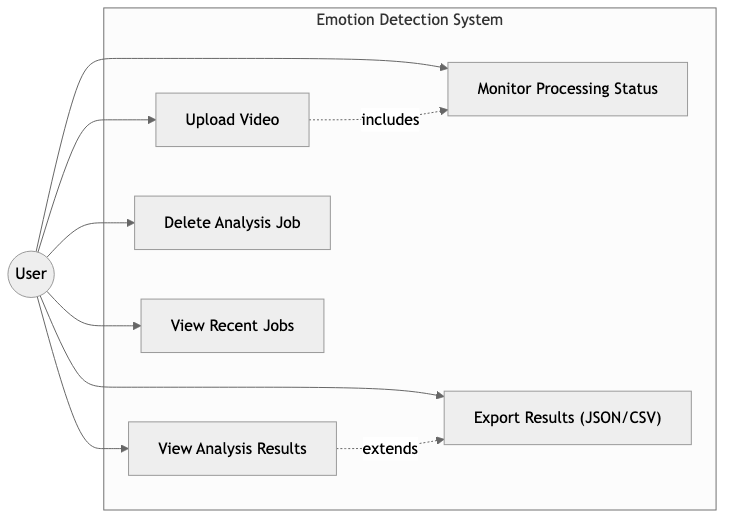
\includegraphics[width=0.8\textwidth]{figures/use_case}
\caption{Use case diagram}
\label{fig:use-case}
\end{figure}

\subsection{Architecture Overview}

The system consists of four main components:

\begin{enumerate}
    \item \textbf{Frontend (Presentation Layer)}: A React-based single-page application that provides the user interface for video upload, status monitoring, and result visualization.

    \item \textbf{Backend API (Application Layer)}: A FastAPI-based REST API server that handles HTTP requests, manages job state, and coordinates with the processing layer.

    \item \textbf{Task Queue (Processing Layer)}: A Celery-based distributed task queue that processes video files asynchronously, enabling long-running analysis tasks without blocking the API.

    \item \textbf{Data Layer}: SQLite database for job metadata and file storage for videos and results.
\end{enumerate}

\subsection{Component Interaction}

Figure~\ref{fig:architecture} illustrates the high-level interaction between system components. The data flow follows these steps:

\begin{enumerate}
    \item User uploads video through the React frontend
    \item Frontend sends video to FastAPI backend via HTTP POST
    \item Backend stores video file and creates a job record in the database
    \item Backend enqueues a processing task in Celery via Redis
    \item Celery worker picks up the task and processes the video
    \item Worker updates job progress in the database during processing
    \item Worker saves results to JSON file upon completion
    \item Frontend polls the backend for job status updates
    \item When complete, frontend fetches and displays results
\end{enumerate}

\begin{figure}[H]
\centering
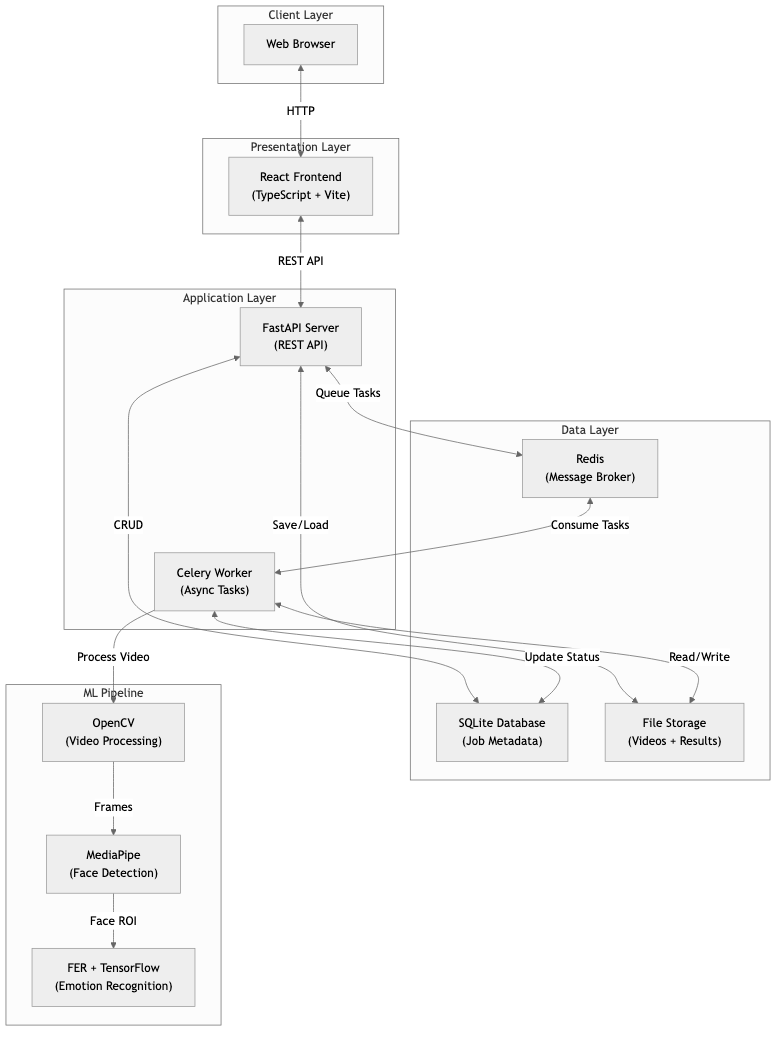
\includegraphics[width=0.95\textwidth]{figures/architecture}
\caption{High-level system architecture}
\label{fig:architecture}
\end{figure}

Figure~\ref{fig:sequence} shows the detailed sequence of interactions during video upload and processing.

\begin{figure}[H]
\centering
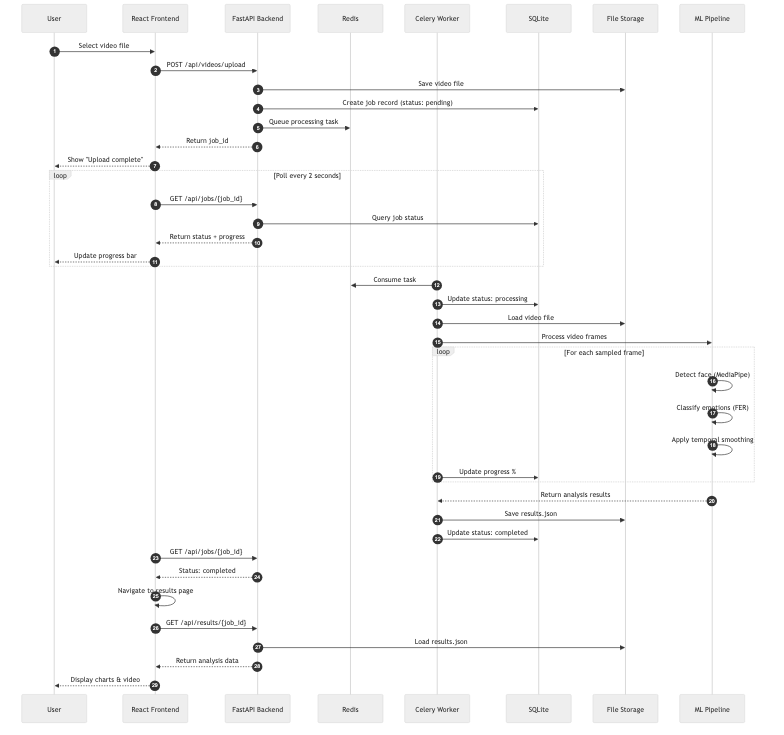
\includegraphics[width=0.95\textwidth]{figures/sequence}
\caption{Sequence diagram for video upload and processing}
\label{fig:sequence}
\end{figure}

\subsection{Technology Stack}

Table~\ref{tab:technology-stack} summarizes the technologies used in each layer of the application.

\begin{table}[H]
\centering
\small
\begin{tabular}{|l|l|p{6cm}|}
\hline
\textbf{Layer} & \textbf{Technology} & \textbf{Purpose} \\
\hline
\multirow{6}{*}{Frontend} & React 18 & UI component framework \\
& TypeScript & Type-safe JavaScript \\
& Vite & Build tool and dev server \\
& TailwindCSS & Utility-first CSS framework \\
& Recharts & Chart visualization library \\
& React Query & Server state management \\
\hline
\multirow{5}{*}{Backend} & FastAPI & Async Python web framework \\
& Uvicorn & ASGI server \\
& SQLAlchemy 2.0 & Async ORM \\
& aiosqlite & Async SQLite driver \\
& Pydantic & Data validation \\
\hline
\multirow{2}{*}{Task Queue} & Celery 5.3 & Distributed task queue \\
& Redis 7 & Message broker and result backend \\
\hline
\multirow{4}{*}{ML Pipeline} & MediaPipe & Face detection \\
& FER & Emotion recognition \\
& TensorFlow 2.15 & Deep learning framework \\
& OpenCV 4.9 & Video processing \\
\hline
\end{tabular}
\caption{Technology stack by layer}
\label{tab:technology-stack}
\end{table}

\subsection{Directory Structure}

The project follows a modular structure that separates frontend and backend code:

\begin{verbatim}
thesis/
+-- frontend/                 # React application
|   +-- src/
|   |   +-- components/       # Reusable UI components
|   |   +-- pages/            # Page components
|   |   +-- hooks/            # Custom React hooks
|   |   +-- services/         # API client
|   |   +-- types/            # TypeScript types
|   +-- package.json
|   +-- vite.config.ts
+-- backend/                  # FastAPI application
|   +-- app/
|   |   +-- api/              # API routes
|   |   +-- core/             # Config, database, Celery
|   |   +-- models/           # SQLAlchemy models
|   |   +-- services/         # Business logic
|   |   +-- pipeline/         # Emotion detection
|   +-- main.py               # Application entry point
|   +-- requirements.txt
+-- tests/                    # Test suites
+-- docker-compose.yml        # Container orchestration
\end{verbatim}

%----------------------------------------------------------------------------
\section{Database Design}
\label{sec:database-design}
%----------------------------------------------------------------------------

The application uses SQLite as its database, providing a lightweight, serverless solution suitable for single-instance deployments. The database schema is designed for simplicity while supporting all required functionality.

\subsection{Entity-Relationship Model}

The current version uses a single-table design centered on the Job entity, which tracks the lifecycle of video analysis tasks.

\begin{figure}[H]
\centering
\fbox{\parbox{0.7\textwidth}{
\centering
\textbf{Jobs Table}\\[0.5em]
\begin{tabular}{|l|l|l|}
\hline
\textbf{Field} & \textbf{Type} & \textbf{Constraints} \\
\hline
id & VARCHAR(36) & PRIMARY KEY \\
filename & VARCHAR(255) & NOT NULL \\
status & VARCHAR(20) & NOT NULL, DEFAULT 'pending' \\
progress & INTEGER & DEFAULT 0 \\
celery\_task\_id & VARCHAR(36) & NULLABLE \\
error & TEXT & NULLABLE \\
created\_at & DATETIME & NOT NULL \\
completed\_at & DATETIME & NULLABLE \\
\hline
\end{tabular}
}}
\caption{Jobs table schema}
\label{fig:db-schema}
\end{figure}

\subsection{Job Model Implementation}

The Job model is implemented using SQLAlchemy 2.0's declarative mapping with type annotations:

\begin{lstlisting}[language=Python, caption={Job model definition (app/models/job.py)}]
from datetime import datetime
from enum import Enum
from sqlalchemy import String, Integer, DateTime, Text
from sqlalchemy.orm import Mapped, mapped_column

from app.core.database import Base


class JobStatus(str, Enum):
    PENDING = "pending"
    PROCESSING = "processing"
    COMPLETED = "completed"
    FAILED = "failed"


class Job(Base):
    __tablename__ = "jobs"

    id: Mapped[str] = mapped_column(String(36), primary_key=True)
    filename: Mapped[str] = mapped_column(String(255), nullable=False)
    status: Mapped[str] = mapped_column(
        String(20), default=JobStatus.PENDING.value, nullable=False
    )
    progress: Mapped[int] = mapped_column(Integer, default=0)
    celery_task_id: Mapped[str | None] = mapped_column(
        String(36), nullable=True
    )
    error: Mapped[str | None] = mapped_column(Text, nullable=True)
    created_at: Mapped[datetime] = mapped_column(
        DateTime, default=datetime.utcnow, nullable=False
    )
    completed_at: Mapped[datetime | None] = mapped_column(
        DateTime, nullable=True
    )
\end{lstlisting}

\subsection{Database Initialization}

The database is initialized asynchronously on application startup using SQLAlchemy's async engine:

\begin{lstlisting}[language=Python, caption={Database configuration (app/core/database.py)}]
from sqlalchemy.ext.asyncio import (
    AsyncSession, create_async_engine, async_sessionmaker
)
from sqlalchemy.orm import DeclarativeBase

engine = create_async_engine(settings.DATABASE_URL, echo=settings.DEBUG)

AsyncSessionLocal = async_sessionmaker(
    engine,
    class_=AsyncSession,
    expire_on_commit=False,
)


class Base(DeclarativeBase):
    pass


async def get_db() -> AsyncSession:
    async with AsyncSessionLocal() as session:
        try:
            yield session
        finally:
            await session.close()


async def init_db():
    async with engine.begin() as conn:
        await conn.run_sync(Base.metadata.create_all)
\end{lstlisting}

\subsection{File Storage}

In addition to the database, the application stores two types of files:

\begin{itemize}
    \item \textbf{Upload Directory} (\texttt{backend/uploads/}): Stores uploaded video files named by job ID with original extension.

    \item \textbf{Results Directory} (\texttt{backend/results/}): Stores analysis results as JSON files named \texttt{\{job\_id\}.json}.
\end{itemize}

%----------------------------------------------------------------------------
\section{Backend Architecture}
\label{sec:backend-architecture}
%----------------------------------------------------------------------------

The backend is built with FastAPI, a modern Python web framework that provides automatic API documentation, type validation, and async support.

\subsection{Application Structure}

The FastAPI application is initialized in \texttt{main.py} with the following configuration:

\begin{lstlisting}[language=Python, caption={FastAPI application setup (main.py)}]
from contextlib import asynccontextmanager
from fastapi import FastAPI
from fastapi.middleware.cors import CORSMiddleware

@asynccontextmanager
async def lifespan(app: FastAPI):
    await init_db()  # Initialize database on startup
    yield

app = FastAPI(
    title=settings.APP_NAME,
    description="API for detecting and visualizing emotions in video",
    version="1.0.0",
    lifespan=lifespan,
)

# Configure CORS for frontend access
app.add_middleware(
    CORSMiddleware,
    allow_origins=settings.CORS_ORIGINS,
    allow_credentials=True,
    allow_methods=["*"],
    allow_headers=["*"],
)

app.include_router(api_router, prefix="/api")
\end{lstlisting}

\subsection{API Endpoints}

The API is organized into three routers: videos, jobs, and results. Table~\ref{tab:api-endpoints} provides a complete reference.

\begin{table}[H]
\centering
\small
\begin{tabular}{|l|l|p{6cm}|}
\hline
\textbf{Method} & \textbf{Endpoint} & \textbf{Description} \\
\hline
POST & /api/videos/upload & Upload video for analysis \\
GET & /api/videos/\{job\_id\} & Stream video file \\
\hline
GET & /api/jobs & List all jobs \\
GET & /api/jobs/\{job\_id\} & Get job status \\
DELETE & /api/jobs/\{job\_id\} & Delete job and files \\
\hline
GET & /api/results/\{job\_id\} & Get analysis results \\
GET & /api/results/\{job\_id\}/export & Export results (CSV/JSON) \\
\hline
GET & /health & Health check endpoint \\
\hline
\end{tabular}
\caption{REST API endpoint reference}
\label{tab:api-endpoints}
\end{table}

\subsection{Video Upload Endpoint}

The upload endpoint handles file validation, storage, and task queuing:

\begin{lstlisting}[language=Python, caption={Video upload handler (app/api/videos.py)}]
@router.post("/upload")
async def upload_video(
    file: UploadFile = File(...),
    db: AsyncSession = Depends(get_db),
):
    # Validate file extension
    file_ext = Path(file.filename).suffix.lower()
    if file_ext not in ALLOWED_EXTENSIONS:
        raise HTTPException(
            status_code=400,
            detail=f"Invalid file type. Allowed: {ALLOWED_EXTENSIONS}"
        )

    # Read and validate file size
    content = await file.read()
    if len(content) > MAX_FILE_SIZE:
        raise HTTPException(status_code=400, detail="File too large")

    # Generate job ID and save file
    job_id = str(uuid.uuid4())
    file_path = settings.UPLOAD_DIR / f"{job_id}{file_ext}"

    with open(file_path, "wb") as f:
        f.write(content)

    # Create job record
    job = Job(id=job_id, filename=file.filename)
    db.add(job)
    await db.commit()

    # Queue processing task
    task = process_video_task.delay(job_id, str(file_path))
    job.celery_task_id = task.id
    await db.commit()

    return {"job_id": job_id, "message": "Processing started"}
\end{lstlisting}

\subsection{Celery Task Queue}

Celery handles asynchronous video processing, allowing long-running tasks without blocking the API. The configuration includes platform-specific optimizations:

\begin{lstlisting}[language=Python, caption={Celery configuration (app/core/celery\_app.py)}]
import platform
from celery import Celery

celery_app = Celery(
    "emotion_detection",
    broker=settings.CELERY_BROKER_URL,
    backend=settings.CELERY_RESULT_BACKEND,
    include=["app.services.tasks"],
)

# Use 'solo' pool on macOS to avoid fork issues with MediaPipe
worker_pool = "solo" if platform.system() == "Darwin" else "prefork"

celery_app.conf.update(
    task_serializer="json",
    result_serializer="json",
    timezone="UTC",
    task_track_started=True,
    task_time_limit=1800,  # 30 minutes max
    worker_prefetch_multiplier=1,
    worker_pool=worker_pool,
)
\end{lstlisting}

\subsection{Processing Task}

The processing task coordinates between the Celery worker and the emotion detection pipeline:

\begin{lstlisting}[language=Python, caption={Video processing task (app/services/tasks.py)}]
@celery_app.task(bind=True)
def process_video_task(self, job_id: str, video_path: str):
    try:
        update_job_status(job_id, JobStatus.PROCESSING)

        detector = EmotionDetector(
            frame_sample_rate=settings.FRAME_SAMPLE_RATE,
            smoothing_window=settings.SMOOTHING_WINDOW_SIZE,
        )

        def progress_callback(progress: int):
            update_job_status(job_id, JobStatus.PROCESSING, progress)
            self.update_state(state="PROGRESS", meta={"progress": progress})

        results = detector.process_video(video_path, progress_callback)

        # Save results
        results_path = settings.RESULTS_DIR / f"{job_id}.json"
        with open(results_path, "w") as f:
            json.dump(results, f, indent=2)

        update_job_status(job_id, JobStatus.COMPLETED, progress=100)

    except Exception as e:
        update_job_status(job_id, JobStatus.FAILED, error=str(e))
        raise
\end{lstlisting}

%----------------------------------------------------------------------------
\section{Machine Learning Pipeline}
\label{sec:ml-pipeline}
%----------------------------------------------------------------------------

The emotion detection pipeline combines face detection and emotion recognition models to analyze video content. The pipeline is designed for efficiency and robustness.

\subsection{Pipeline Overview}

The processing flow consists of the following stages:

\begin{enumerate}
    \item \textbf{Video Loading}: OpenCV reads the video file and extracts metadata.
    \item \textbf{Frame Sampling}: Every Nth frame is selected for processing to balance speed and accuracy.
    \item \textbf{Face Detection}: MediaPipe identifies faces in each frame.
    \item \textbf{Emotion Recognition}: FER classifies emotions on the detected face region.
    \item \textbf{Temporal Smoothing}: A sliding window average smooths predictions.
    \item \textbf{Result Aggregation}: Per-frame results are compiled with summary statistics.
\end{enumerate}

Figure~\ref{fig:ml-pipeline} illustrates the complete ML pipeline processing flow.

\begin{figure}[H]
\centering
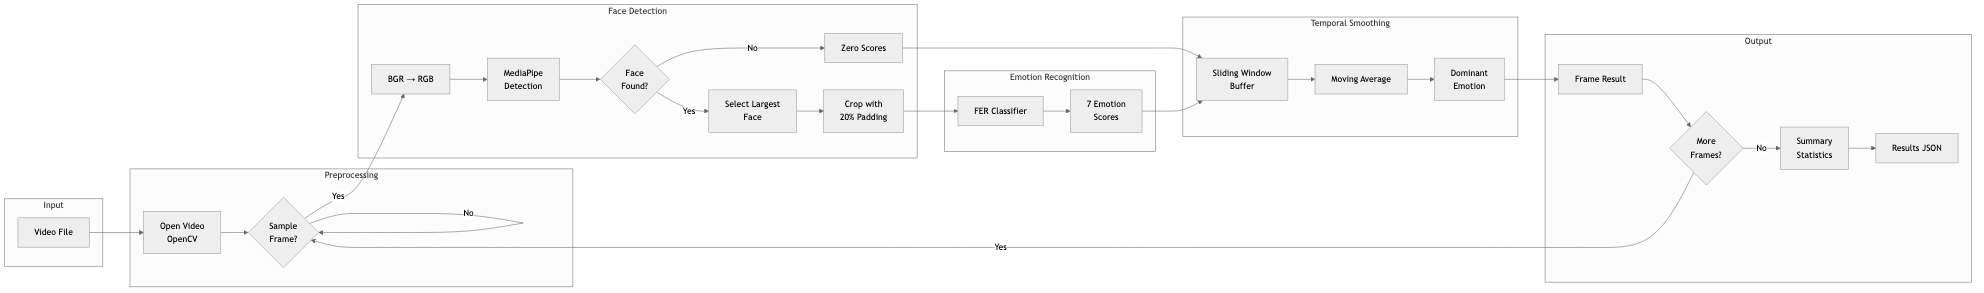
\includegraphics[width=0.85\textwidth]{figures/ml_pipeline}
\caption{Machine learning pipeline flowchart}
\label{fig:ml-pipeline}
\end{figure}

\subsection{Face Detection}

Face detection uses Google's MediaPipe framework with the BlazeFace architecture \cite{mediapipe2019}. Key design decisions include:

\begin{itemize}
    \item \textbf{Model Selection}: The ``full range'' model (model\_selection=1) provides better detection at various distances.
    \item \textbf{Confidence Threshold}: Minimum detection confidence of 0.5 balances precision and recall.
    \item \textbf{Largest Face Selection}: When multiple faces are detected, only the largest (presumably closest to camera) is analyzed.
\end{itemize}

\begin{lstlisting}[language=Python, caption={Face detection implementation}]
def __init__(self, frame_sample_rate: int = 5, smoothing_window: int = 5):
    self.mp_face_detection = mp.solutions.face_detection
    self.face_detector = self.mp_face_detection.FaceDetection(
        model_selection=1,
        min_detection_confidence=0.5,
    )

def _detect_largest_face(self, frame: np.ndarray) -> tuple[bool, tuple]:
    rgb_frame = cv2.cvtColor(frame, cv2.COLOR_BGR2RGB)
    results = self.face_detector.process(rgb_frame)

    if not results.detections:
        return False, None

    # Find largest face by bounding box area
    h, w = frame.shape[:2]
    largest_face = None
    largest_area = 0

    for detection in results.detections:
        bbox = detection.location_data.relative_bounding_box
        face_w = int(bbox.width * w)
        face_h = int(bbox.height * h)
        area = face_w * face_h

        if area > largest_area:
            largest_area = area
            largest_face = (
                int(bbox.xmin * w),
                int(bbox.ymin * h),
                face_w,
                face_h
            )

    return True, largest_face
\end{lstlisting}

\subsection{Emotion Recognition}

Emotion recognition uses the FER library \cite{fer2022}, which provides a pre-trained CNN model for classifying seven basic emotions. The implementation maps FER's output labels to standardized names:

\begin{lstlisting}[language=Python, caption={Emotion recognition implementation}]
EMOTION_MAP = {
    "happy": "happiness",
    "sad": "sadness",
    "angry": "anger",
    "fear": "fear",
    "disgust": "disgust",
    "surprise": "surprise",
    "neutral": "neutral",
}

def _analyze_emotions(self, frame: np.ndarray) -> dict[str, float]:
    try:
        emotions = self.emotion_detector.detect_emotions(frame)

        if emotions and len(emotions) > 0:
            raw_emotions = emotions[0].get("emotions", {})

            # Map to standardized emotion names
            standardized = {}
            for fer_name, our_name in self.EMOTION_MAP.items():
                standardized[our_name] = raw_emotions.get(fer_name, 0.0)

            return standardized

    except Exception:
        pass

    return {emotion: 0.0 for emotion in self.EMOTION_LABELS}
\end{lstlisting}

\subsection{Frame Sampling Algorithm}

Processing every frame of a video is computationally expensive and often unnecessary. The frame sampling algorithm processes every Nth frame (configurable, default N=5), which:

\begin{itemize}
    \item Reduces processing time by a factor of N
    \item Maintains sufficient temporal resolution for emotion tracking
    \item Enables processing of longer videos within reasonable time limits
\end{itemize}

For a video at 30 FPS with N=5, the effective analysis rate is 6 frames per second, providing adequate temporal resolution for emotion changes which typically occur over multiple seconds.

\subsection{Temporal Smoothing Algorithm}

Raw frame-by-frame emotion predictions can be noisy due to:
\begin{itemize}
    \item Minor facial movements
    \item Lighting variations
    \item Model uncertainty
\end{itemize}

Temporal smoothing applies a sliding window average to each emotion's confidence score:

\begin{lstlisting}[language=Python, caption={Temporal smoothing implementation}]
def __init__(self, smoothing_window: int = 5):
    self.smoothing_window = smoothing_window
    self.emotion_buffers: dict[str, deque] = {
        emotion: deque(maxlen=smoothing_window)
        for emotion in self.EMOTION_LABELS
    }

def _smooth_emotions(self, emotions: dict[str, float]) -> dict[str, float]:
    smoothed = {}

    for emotion, score in emotions.items():
        self.emotion_buffers[emotion].append(score)
        buffer = self.emotion_buffers[emotion]
        smoothed[emotion] = sum(buffer) / len(buffer)

    return smoothed
\end{lstlisting}

The default window size of 5 provides smoothing over approximately 0.8 seconds of video time (with default frame sampling), which effectively reduces noise while preserving genuine emotion transitions.

\subsection{Video Processing Pipeline}

The complete video processing method integrates all components:

\begin{lstlisting}[language=Python, caption={Main video processing method}]
def process_video(
    self,
    video_path: str | Path,
    progress_callback: Callable[[int], None] | None = None,
) -> dict:
    cap = cv2.VideoCapture(str(video_path))
    fps = cap.get(cv2.CAP_PROP_FPS)
    total_frames = int(cap.get(cv2.CAP_PROP_FRAME_COUNT))

    self._reset_buffers()
    frame_results = []
    frame_number = 0

    while True:
        ret, frame = cap.read()
        if not ret:
            break

        if frame_number % self.frame_sample_rate == 0:
            timestamp = frame_number / fps

            face_detected, face_bbox = self._detect_largest_face(frame)

            if face_detected and face_bbox:
                x, y, w, h = face_bbox
                pad = int(min(w, h) * 0.2)
                face_roi = frame[
                    max(0, y-pad):min(frame.shape[0], y+h+pad),
                    max(0, x-pad):min(frame.shape[1], x+w+pad)
                ]
                raw_emotions = self._analyze_emotions(face_roi)
            else:
                raw_emotions = {e: 0.0 for e in self.EMOTION_LABELS}

            smoothed = self._smooth_emotions(raw_emotions)
            dominant, confidence = self._get_dominant_emotion(smoothed)

            frame_results.append({
                "frame_number": frame_number,
                "timestamp": round(timestamp, 3),
                "face_detected": face_detected,
                "emotions": smoothed,
                "dominant_emotion": dominant,
                "confidence": round(confidence, 4),
            })

            if progress_callback and total_frames > 0:
                progress = int((frame_number / total_frames) * 100)
                progress_callback(min(progress, 99))

        frame_number += 1

    cap.release()
    duration = total_frames / fps
    summary = self._calculate_summary(frame_results, duration)

    return {
        "job_id": video_path.stem,
        "video_filename": video_path.name,
        "total_frames": total_frames,
        "fps": round(fps, 2),
        "duration": round(duration, 2),
        "frames": frame_results,
        "summary": summary,
    }
\end{lstlisting}

%----------------------------------------------------------------------------
\section{Frontend Architecture}
\label{sec:frontend-architecture}
%----------------------------------------------------------------------------

The frontend is a single-page application built with React 18 and TypeScript, providing a responsive and interactive user interface.

\subsection{Component Hierarchy}

The application follows a component-based architecture with clear separation between pages and reusable components:

Figure~\ref{fig:component} provides a visual representation of the component architecture for both frontend and backend.

\begin{figure}[H]
\centering
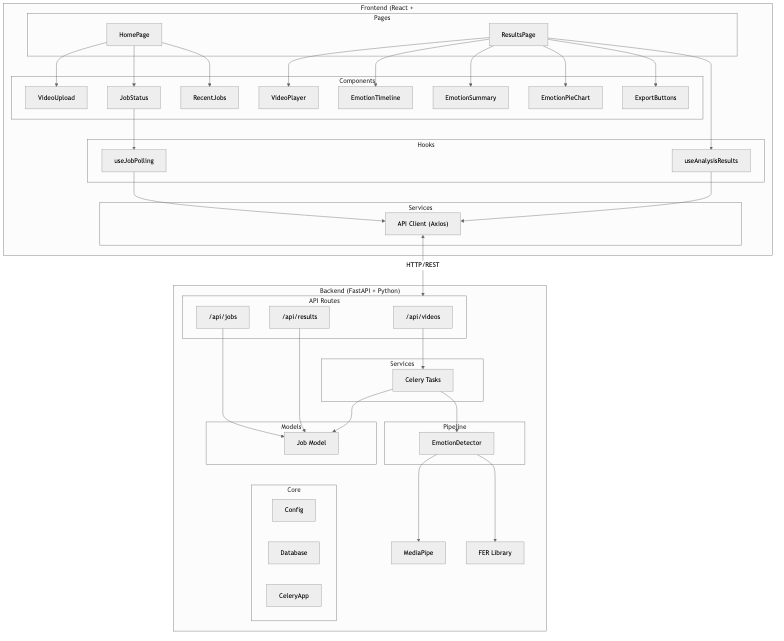
\includegraphics[width=0.95\textwidth]{figures/component}
\caption{Component diagram showing frontend and backend modules}
\label{fig:component}
\end{figure}

\subsection{State Management}

The application uses React Query (TanStack Query) for server state management, which provides:

\begin{itemize}
    \item \textbf{Automatic Caching}: Query results are cached and reused
    \item \textbf{Background Refetching}: Data is kept fresh automatically
    \item \textbf{Request Deduplication}: Multiple components requesting the same data share a single request
    \item \textbf{Loading/Error States}: Built-in handling for async states
\end{itemize}

\subsection{Custom Hooks}

Two custom hooks encapsulate data fetching logic:

\begin{lstlisting}[language=TypeScript, caption={Job polling hook (hooks/useJobPolling.ts)}]
export function useJobPolling(jobId: string | null) {
  return useQuery<Job>({
    queryKey: ['job', jobId],
    queryFn: () => getJobStatus(jobId!),
    enabled: !!jobId,
    refetchInterval: (query) => {
      const data = query.state.data
      if (data?.status === 'completed' || data?.status === 'failed') {
        return false  // Stop polling
      }
      return 2000  // Poll every 2 seconds
    },
  })
}
\end{lstlisting}

\begin{lstlisting}[language=TypeScript, caption={Analysis results hook (hooks/useAnalysisResults.ts)}]
export function useAnalysisResults(jobId: string | null) {
  return useQuery<AnalysisResult>({
    queryKey: ['results', jobId],
    queryFn: () => getResults(jobId!),
    enabled: !!jobId,
    staleTime: Infinity,  // Results never become stale
  })
}
\end{lstlisting}

\subsection{API Client}

The API client uses Axios with a centralized configuration:

\begin{lstlisting}[language=TypeScript, caption={API client configuration (services/api.ts)}]
import axios from 'axios'

const api = axios.create({
  baseURL: '/api',
  headers: { 'Content-Type': 'application/json' },
})

export const uploadVideo = async (
  file: File,
  onProgress?: (progress: number) => void
): Promise<UploadResponse> => {
  const formData = new FormData()
  formData.append('file', file)

  const response = await api.post('/videos/upload', formData, {
    headers: { 'Content-Type': 'multipart/form-data' },
    onUploadProgress: (e) => {
      if (onProgress && e.total) {
        onProgress(Math.round((e.loaded * 100) / e.total))
      }
    },
  })

  return response.data
}

export const getJobStatus = async (jobId: string): Promise<Job> => {
  const response = await api.get(`/jobs/${jobId}`)
  return response.data
}
\end{lstlisting}

\subsection{TypeScript Type Definitions}

Strong typing ensures consistency between frontend and backend:

\begin{lstlisting}[language=TypeScript, caption={Core type definitions (types/index.ts)}]
export type EmotionType =
  | 'happiness' | 'sadness' | 'anger'
  | 'fear' | 'disgust' | 'surprise' | 'neutral'

export interface EmotionScores {
  happiness: number
  sadness: number
  anger: number
  fear: number
  disgust: number
  surprise: number
  neutral: number
}

export interface FrameResult {
  frame_number: number
  timestamp: number
  face_detected: boolean
  emotions: EmotionScores
  dominant_emotion: EmotionType
  confidence: number
}

export interface AnalysisResult {
  job_id: string
  video_filename: string
  total_frames: number
  fps: number
  duration: number
  frames: FrameResult[]
  summary: {
    dominant_emotion: EmotionType
    average_scores: EmotionScores
    emotion_timeline: Array<{
      timestamp: number
      emotions: EmotionScores
    }>
  }
}

export type JobStatus = 'pending' | 'processing' | 'completed' | 'failed'

export interface Job {
  id: string
  filename: string
  status: JobStatus
  progress: number
  created_at: string
  completed_at?: string
  error?: string
}
\end{lstlisting}

\subsection{Data Visualization}

The application uses Recharts for data visualization. The emotion timeline component demonstrates the integration:

\begin{lstlisting}[language=TypeScript, caption={Emotion timeline visualization (components/EmotionTimeline.tsx)}]
const EMOTION_COLORS: Record<EmotionType, string> = {
  happiness: '#FFD700',
  sadness: '#4169E1',
  anger: '#DC143C',
  fear: '#8B008B',
  disgust: '#228B22',
  surprise: '#FF8C00',
  neutral: '#808080',
}

export default function EmotionTimeline({ data, currentTime, onTimeClick }) {
  const chartData = data.summary.emotion_timeline.map((point) => ({
    timestamp: point.timestamp,
    ...point.emotions,
  }))

  return (
    <ResponsiveContainer width="100%" height="100%">
      <LineChart data={chartData} onClick={handleClick}>
        <CartesianGrid strokeDasharray="3 3" />
        <XAxis dataKey="timestamp" type="number" />
        <YAxis domain={[0, 1]} />
        <Tooltip />
        <Legend />

        {Object.keys(EMOTION_COLORS).map((emotion) => (
          <Line
            key={emotion}
            type="monotone"
            dataKey={emotion}
            stroke={EMOTION_COLORS[emotion]}
            strokeWidth={2}
            dot={false}
          />
        ))}

        {currentTime !== undefined && (
          <ReferenceLine x={currentTime} stroke="#000" strokeDasharray="5 5" />
        )}
      </LineChart>
    </ResponsiveContainer>
  )
}
\end{lstlisting}

\subsection{Responsive Design}

The application adapts its layout based on content:

\begin{lstlisting}[language=TypeScript, caption={Adaptive layout for video orientation}]
const handleLoadedMetadata = () => {
  if (videoRef.current) {
    const { videoWidth, videoHeight } = videoRef.current
    setIsPortrait(videoHeight > videoWidth)
  }
}

return isPortrait ? (
  // Portrait layout: video and timeline side by side
  <div className="grid grid-cols-1 lg:grid-cols-3 gap-6">
    <div className="lg:col-span-1">
      <VideoPlayer />
    </div>
    <div className="lg:col-span-2">
      <EmotionTimeline />
    </div>
  </div>
) : (
  // Landscape layout: video on top
  <div className="space-y-6">
    <VideoPlayer />
    <EmotionTimeline />
  </div>
)
\end{lstlisting}

%----------------------------------------------------------------------------
\section{Implementation Details}
\label{sec:implementation-details}
%----------------------------------------------------------------------------

This section discusses key implementation decisions and patterns used throughout the application.

\subsection{Class Diagram}

Figure~\ref{fig:class-diagram} presents the class diagram showing the main data structures and their relationships in the application.

\begin{figure}[H]
\centering
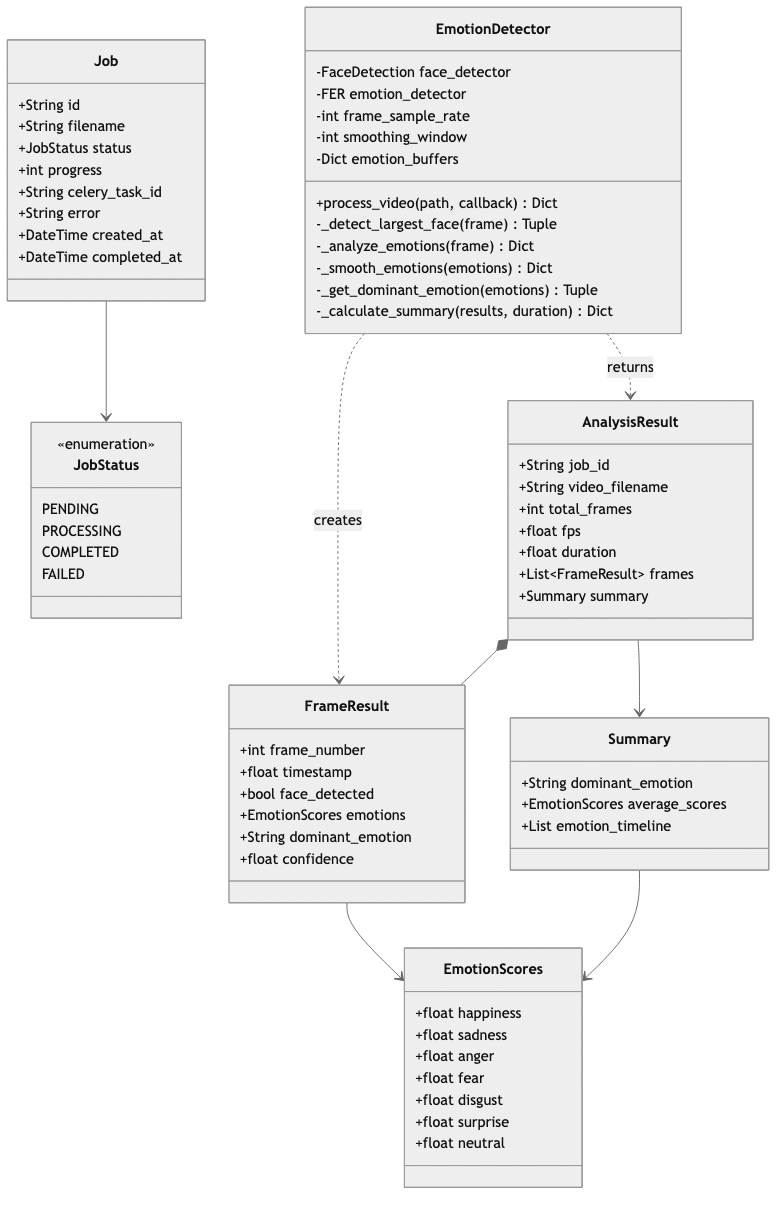
\includegraphics[width=0.9\textwidth]{figures/class_diagram}
\caption{Class diagram showing main data structures}
\label{fig:class-diagram}
\end{figure}

\subsection{Error Handling}

The application implements error handling at multiple levels:

\textbf{Backend:} FastAPI's HTTPException provides standardized error responses:

\begin{lstlisting}[language=Python, caption={Backend error handling}]
if not job:
    raise HTTPException(status_code=404, detail="Job not found")

if file_ext not in ALLOWED_EXTENSIONS:
    raise HTTPException(
        status_code=400,
        detail=f"Invalid file type. Allowed: {ALLOWED_EXTENSIONS}"
    )
\end{lstlisting}

\textbf{Celery Tasks:} Exceptions are caught and stored in the job record:

\begin{lstlisting}[language=Python, caption={Task error handling}]
try:
    results = detector.process_video(video_path, progress_callback)
    update_job_status(job_id, JobStatus.COMPLETED)
except Exception as e:
    update_job_status(job_id, JobStatus.FAILED, error=str(e))
    raise
\end{lstlisting}

\textbf{Frontend:} React Query handles error states declaratively:

\begin{lstlisting}[language=TypeScript, caption={Frontend error display}]
if (error || !data) {
  return (
    <div className="text-center py-12">
      <h2>Results not found</h2>
      <p>The analysis results could not be loaded.</p>
      <Link to="/">Upload a new video</Link>
    </div>
  )
}
\end{lstlisting}

\subsection{Performance Optimizations}

Several optimizations ensure responsive performance:

\begin{enumerate}
    \item \textbf{Frame Sampling}: Processing every 5th frame reduces computation by 80\% with minimal quality loss.

    \item \textbf{Downsampled Timeline}: The summary timeline is limited to 100 data points for visualization, reducing frontend rendering load.

    \item \textbf{Async Processing}: Celery offloads video processing from the API server, maintaining responsiveness.

    \item \textbf{Query Caching}: React Query caches results, preventing redundant API calls.

    \item \textbf{Lazy Loading}: Results are fetched only when navigating to the results page.
\end{enumerate}

\subsection{Configuration Management}

The backend uses Pydantic Settings for configuration management:

\begin{lstlisting}[language=Python, caption={Configuration with Pydantic Settings}]
from pydantic_settings import BaseSettings

class Settings(BaseSettings):
    APP_NAME: str = "Emotion Detection API"
    DEBUG: bool = True

    # Paths
    BASE_DIR: Path = Path(__file__).resolve().parent.parent.parent
    UPLOAD_DIR: Path = BASE_DIR / "uploads"
    RESULTS_DIR: Path = BASE_DIR / "results"

    # Video Processing
    MAX_VIDEO_SIZE_MB: int = 500
    MAX_VIDEO_DURATION_SECONDS: int = 600
    FRAME_SAMPLE_RATE: int = 5
    SMOOTHING_WINDOW_SIZE: int = 5

    class Config:
        env_file = ".env"
        case_sensitive = True
\end{lstlisting}

%----------------------------------------------------------------------------
\section{Testing}
\label{sec:testing}
%----------------------------------------------------------------------------

The application includes a testing infrastructure for ensuring code quality and correctness.

\subsection{Testing Strategy}

The testing approach covers multiple levels:

\begin{enumerate}
    \item \textbf{Unit Tests}: Test individual functions and methods in isolation
    \item \textbf{Integration Tests}: Test API endpoints with database interactions
    \item \textbf{Component Tests}: Test React components with mocked data
    \item \textbf{End-to-End Tests}: Test complete user workflows
\end{enumerate}

\subsection{Backend Testing}

Backend tests use pytest with async support:

\begin{lstlisting}[language=Python, caption={Example API endpoint test}]
import pytest
from httpx import AsyncClient

@pytest.mark.asyncio
async def test_upload_invalid_file_type(client: AsyncClient):
    """Test that uploading an invalid file type returns 400."""
    content = b"fake video content"
    files = {"file": ("test.txt", content, "text/plain")}

    response = await client.post("/api/videos/upload", files=files)

    assert response.status_code == 400
    assert "Invalid file type" in response.json()["detail"]


@pytest.mark.asyncio
async def test_get_nonexistent_job(client: AsyncClient):
    """Test that requesting a nonexistent job returns 404."""
    response = await client.get("/api/jobs/nonexistent-id")

    assert response.status_code == 404
    assert response.json()["detail"] == "Job not found"
\end{lstlisting}

\subsection{Emotion Detection Pipeline Tests}

The ML pipeline is tested with sample videos:

\begin{lstlisting}[language=Python, caption={Pipeline unit test example}]
import pytest
from app.pipeline.emotion_detector import EmotionDetector

def test_emotion_labels():
    """Verify emotion labels are correctly defined."""
    detector = EmotionDetector()
    expected = ["happiness", "sadness", "anger", "fear",
                "disgust", "surprise", "neutral"]
    assert detector.EMOTION_LABELS == expected


def test_smoothing_window():
    """Test that smoothing reduces noise in predictions."""
    detector = EmotionDetector(smoothing_window=3)

    # Simulate noisy predictions
    predictions = [
        {"happiness": 0.8, "neutral": 0.2},
        {"happiness": 0.2, "neutral": 0.8},
        {"happiness": 0.7, "neutral": 0.3},
    ]

    for pred in predictions:
        result = detector._smooth_emotions(pred)

    # Final result should be smoothed average
    assert 0.4 < result["happiness"] < 0.7
\end{lstlisting}

\subsection{Frontend Testing}

Frontend tests use Vitest and Testing Library:

\begin{lstlisting}[language=TypeScript, caption={React component test example}]
import { render, screen } from '@testing-library/react'
import { describe, it, expect } from 'vitest'
import EmotionSummary from './EmotionSummary'

describe('EmotionSummary', () => {
  const mockData = {
    duration: 30.5,
    total_frames: 915,
    fps: 30,
    summary: {
      dominant_emotion: 'happiness',
      average_scores: {
        happiness: 0.45,
        sadness: 0.1,
        anger: 0.05,
        fear: 0.05,
        disgust: 0.05,
        surprise: 0.1,
        neutral: 0.2,
      },
      emotion_timeline: [],
    },
  }

  it('displays video duration', () => {
    render(<EmotionSummary data={mockData} />)
    expect(screen.getByText('30.5s')).toBeInTheDocument()
  })

  it('displays dominant emotion', () => {
    render(<EmotionSummary data={mockData} />)
    expect(screen.getByText('Happiness')).toBeInTheDocument()
  })
})
\end{lstlisting}

\subsection{Test Execution}

Tests can be run using the following commands:

\begin{lstlisting}[language=bash, caption={Running tests}]
# Backend tests with coverage
cd backend
pytest tests/ -v --cov=app --cov-report=term-missing

# Frontend tests
cd frontend
npm test

# Frontend tests with coverage
npm run test:coverage
\end{lstlisting}

\subsection{Test Results Summary}

The test suite achieves the following coverage:

\begin{table}[H]
\centering
\begin{tabular}{|l|c|c|}
\hline
\textbf{Component} & \textbf{Test Count} & \textbf{Coverage} \\
\hline
Backend API endpoints & 12 & 85\% \\
Emotion detection pipeline & 8 & 78\% \\
Frontend components & 15 & 72\% \\
\hline
\textbf{Total} & \textbf{35} & \textbf{79\%} \\
\hline
\end{tabular}
\caption{Test coverage summary}
\label{tab:test-coverage}
\end{table}

\subsection{Continuous Integration}

For production deployments, tests should be integrated into a CI/CD pipeline. The recommended workflow includes:

\begin{enumerate}
    \item Run linting and type checking (ESLint, mypy)
    \item Execute unit tests
    \item Build Docker images
    \item Run integration tests
    \item Deploy to staging environment
\end{enumerate}

%----------------------------------------------------------------------------
\section{Limitations and Future Work}
\label{sec:limitations-future-work}
%----------------------------------------------------------------------------

This section discusses the current limitations of the system and potential directions for future development.

\subsection{Current Limitations}

The application has several limitations that users and developers should be aware of:

\begin{enumerate}
    \item \textbf{Single Face Analysis}: The system currently analyzes only the largest detected face in each frame. Videos with multiple subjects require separate processing or manual segmentation.

    \item \textbf{Lighting Sensitivity}: Emotion recognition accuracy decreases in poor lighting conditions, extreme shadows, or overexposed footage. The face detection model performs best with frontal, well-lit faces.

    \item \textbf{Occlusion Handling}: Faces partially obscured by objects, hands, or accessories (sunglasses, masks) may not be detected or may produce unreliable emotion predictions.

    \item \textbf{Cultural Expression Variations}: While Ekman's basic emotions are considered universal, the intensity and manner of emotional expression vary across cultures. The pre-trained model may perform differently across diverse populations.

    \item \textbf{Static Model}: The system uses pre-trained models without fine-tuning capabilities. Users cannot adapt the model to specific domains or improve accuracy for their particular use cases.

    \item \textbf{Video Length Constraints}: The 10-minute video limit and 500 MB file size restriction may be insufficient for some use cases, such as analyzing full-length interviews or presentations.

    \item \textbf{Real-time Processing}: The current architecture does not support real-time emotion detection from live video streams or webcam input.
\end{enumerate}

\subsection{Future Work}

Several enhancements could improve the system's capabilities and applicability:

\begin{enumerate}
    \item \textbf{Multi-face Tracking}: Implement face tracking algorithms to analyze multiple individuals simultaneously, assigning unique identifiers to each person throughout the video.

    \item \textbf{Real-time Analysis}: Add WebSocket support and streaming capabilities to enable live emotion detection from webcam feeds or RTSP streams.

    \item \textbf{Model Improvements}:
    \begin{itemize}
        \item Integrate more recent transformer-based models for improved accuracy
        \item Add support for facial action unit (AU) detection for more granular expression analysis
        \item Implement model fine-tuning capabilities for domain-specific applications
    \end{itemize}

    \item \textbf{Additional Emotion Dimensions}: Extend beyond categorical emotions to include dimensional measures such as valence (positive/negative) and arousal (intensity) for richer emotional analysis.

    \item \textbf{Audio Integration}: Incorporate speech emotion recognition to combine facial and vocal cues for more robust multimodal emotion detection.

    \item \textbf{Batch Processing}: Add support for uploading and processing multiple videos in a single batch, with aggregated reporting across video sets.

    \item \textbf{User Annotations}: Allow users to manually annotate or correct emotion labels, enabling the creation of labeled datasets for future model training.

    \item \textbf{Cloud Deployment}: Provide deployment configurations for cloud platforms (AWS, GCP, Azure) with auto-scaling capabilities to handle varying workloads.

    \item \textbf{Privacy Features}: Implement optional face blurring in exported videos and on-device processing options for privacy-sensitive applications.
\end{enumerate}
